%
%##########################
%# LIENS INTER-PROFILS
%##########################

\subsubsection{Liens entre profils pré et post-opératoires}

Pour comparer les résultats précédents et les profils identifiés, nous reprenons et rapprochons pour chaque patient son profil pré-opératoire et son profil post-opératoire. La liste des couples de profils ainsi obtenue
est triée
\begin{itemize}
 \item  par profil pré-opératoire~: figure~\ref{fig-rtupb-histogram} et figure~\ref{fig-vppbs-histogram} pour respectivement RTUPB et VPPBS
 \item  par profil post-opératoire~: figure~\ref{fig-rtupb-histogram2} et figure~\ref{fig-vppbs-histogram2} pour respectivement RTUPB et VPPBS
\end{itemize}

\begin{figure}[H]
\centering
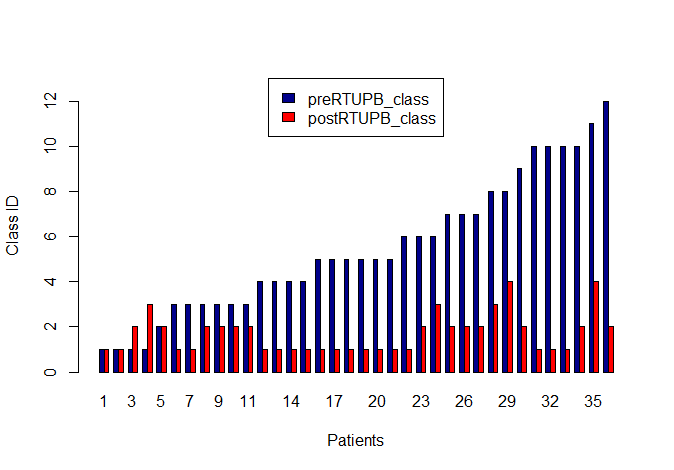
\includegraphics[width=0.75\textwidth]{../Fig/RTUPB/rtupb-histogram-pre-post.png}
\caption{RTUPB: classes post-opératoires en fonction des classes pré-opératoires}
\label{fig-rtupb-histogram}
\end{figure}

La figure~\ref{fig-rtupb-histogram} révèle que pour les patients appartenant au profil pré-opératoire 4, 5 et 7 le résultat constaté est toujours le profil post-opératoire n°1.  Pour les autres profils pré-opératoires (à l'exception des singletons pour lesquels les résultats ne sont donc pas confirmés), il n'existe pas de profils post-opératoires uniques permettant d'en déduire une prévision de guérison.
La figure~\ref{fig-rtupb-histogram2} n'apporte pas d'informations complémentaires.

\begin{figure}[H]
\centering
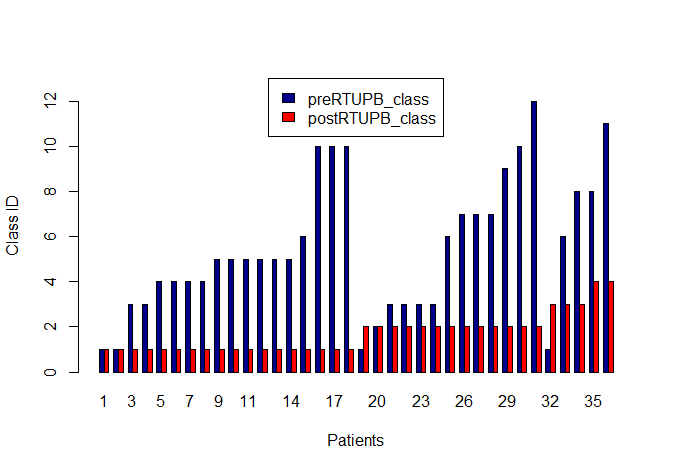
\includegraphics[width=0.75\textwidth]{../Fig/RTUPB/rtupb-histogram-post-pre.png}
\caption{RTUPB: classes pré-opératoires en fonction des classes post-opératoires}
\label{fig-rtupb-histogram2}
\end{figure}

Pour VPPBS, la figure~\ref{fig-vppbs-histogram} montre la correspondance d'un seul profil post-opératoire pour chaque profil pré-opératoire. Nous pouvons donc nous baser sur le profil pré-opératoire pour envisager ou non une opération VPPBS et prévoir la guérison.

\begin{figure}[H]
\centering
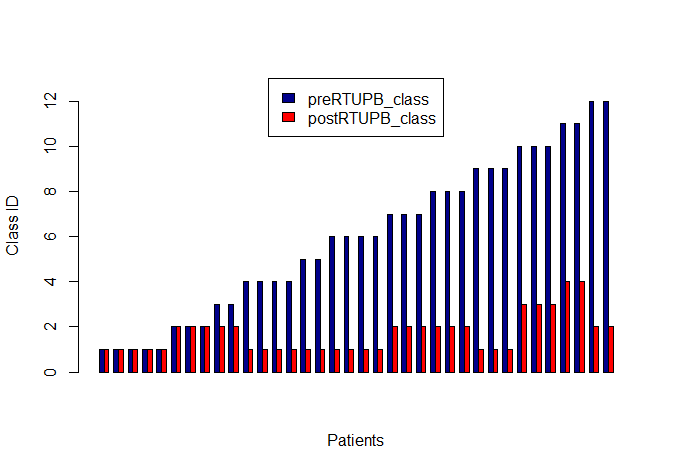
\includegraphics[width=0.75\textwidth]{../Fig/VPPBS/vppbs-histogram-pre-post.png}
\caption{VPPBS: classes post-opératoires en fonction des classes pré-opératoires}
\label{fig-vppbs-histogram}
\end{figure}

\begin{figure}[H]
\centering
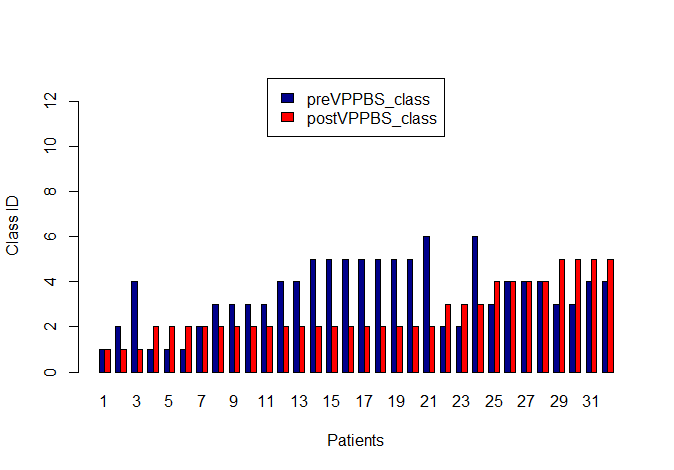
\includegraphics[width=0.75\textwidth]{../Fig/VPPBS/vppbs-histogram-post-pre.png}
\caption{VPPBS: classes pré-opératoires en fonction des classes post-opératoires}
\label{fig-vppbs-histogram2}
\end{figure}
